\chapter{Process model requirements}
\label{ch:processmodels}

In the previous chapters of this dissertation, we have focused on investigating innovation ecosystems as networks with a visual network analytics approach. In order to increase the level of automation in conducting the investigations, we will now move to discuss the process that is required to implement an investigation.

This chapter constructs the basis for the development of a process model for data-driven visual network analytics. We draw from two complementing sources. First, we describe previous work on data-driven visual network analytics and review existing related process models. Second, we identify a set of key requirements that stem from the series of investigations presented in Chapter~\ref{ch:experiments}.

\section{Data-driven visual network analytics}

Data-driven visual network analytics leverages computation to analyze potentially very large datasets in order to identify the structural patterns underlying in a complex phenomenon. The investigations of such phenomenon are further complicated because data on the actors and their transactions often come from multiple and diverse data sources, some of which are not developed for computational use. Especially in cases involving data that are heterogeneous by nature, an iterative, incremental analysis process is sometimes necessary \citep{Telea2008}. Analysis of complex phenomena often involves multiple pathways to actionable recommendations, and assumptions underlying decisions may change over time.

We agree with \cite{Freeman2000VisualizingNetworks} in that integrated tools that can be used to collect, manage and visualize the SNA data are key in supporting network investigations \cite[cf.][]{Huhtamaki2010Context-DrivenCo-Creation}. The tradeoff between usability and automation sometimes creates a barrier for new entrants into data-driven visual network analysis \citep{Hansen2012DoData}.

A gap exists between the vision of easy-to-use integrated tools and the practice of data-driven visual network analytics, however. Data available for analysis is, for a number of reasons, notoriously difficult to process \citep{Salonen2013ChallengesMedia}. Individual investigators or  small investigative teams often use manual processes or rely on ready-made tools that are operated through graphical user interfaces. Using these stand-alone tools is very straightforward. The available data sources and analysis and visualization functionalities are, however, somewhat limited. On the other side of the spectrum, the full-stack, programming-centric processes, in which massive sets of data are mined with tools that are developed and operated by experts, are generally run in complex cloud-based environments.

\section{Review of existing process models}

Several process models with different levels of abstraction exist to give structure to data-driven, visualization-centric investigations. In the next section, we will review a selection of the existing process models. The review follows \ref{pub:ostinato} \citep{Huhtamaki2015Ostinato:Analytics}.

Our approach into data-driven visual network analytics builds on a number of pieces of knowledge including 
information visualization \citep{Card1999ReadingsThink}, 
data-driven visualization pipelines \citep{Nykanen2008}, 
interactive network analysis \citep{Hansen2012DoData},
visual analytics \citep{Wong2004VisualAnalytics},
sensemaking \citep{Pirolli2005TheAnalysis, Weick2005OrganizingSensemaking},
interactive visualization \citep{Heer2012InteractiveAnalysis} and 
scientific visualization \citep{Telea2008}. All these approaches introduce models and pose key requirements that should be considered when developing next-generation tools and toolchains for visual network analytics. Moreover, the objective to conduct and publish research in a reproducible way \citep{Peng2009,Peng2011, Ghosh2013} contributes to the overall quality of the analytics process and also introduces additional requirements.

To support the use of network analysis, \cite{Hansen2012DoData} build on top of the sensemaking model \citep{Pirolli2005TheAnalysis} to present Network Analysis and Visualization (NAV), a process model to support novices that enter network analysis. The NAV process starts with defining the goals for the analysis and continues through data collection and structuring, after which data are interpreted through multiple loops of network visualization and SNA metrics calculation. Finally, the insights and conclusions are formatted and summarized, then disseminated through a report. Seeking low-barrier entry, \cite{Hansen2011AnalyzingWorld} introduce NodeXL, an Excel-based toolset for SNA, to conduct the analysis and define ways to apply these metrics in investigating phenomena taking place in social media.

\cite{Card1999ReadingsThink} present the information visualization reference model, a four-step process that can be used as a blueprint for implementing data-driven visualization processes. First, raw data is collected and, second, refined into data tables to allow straightforward processing. Third, data tables are transformed into a portfolio of visual representations from which various concrete views are, fourth, served to the visualization user for sensemaking. Imperatively, the reference model suggests that best practice is when the user can interact with all steps of the process.

\begin{figure}[htb]
\centering
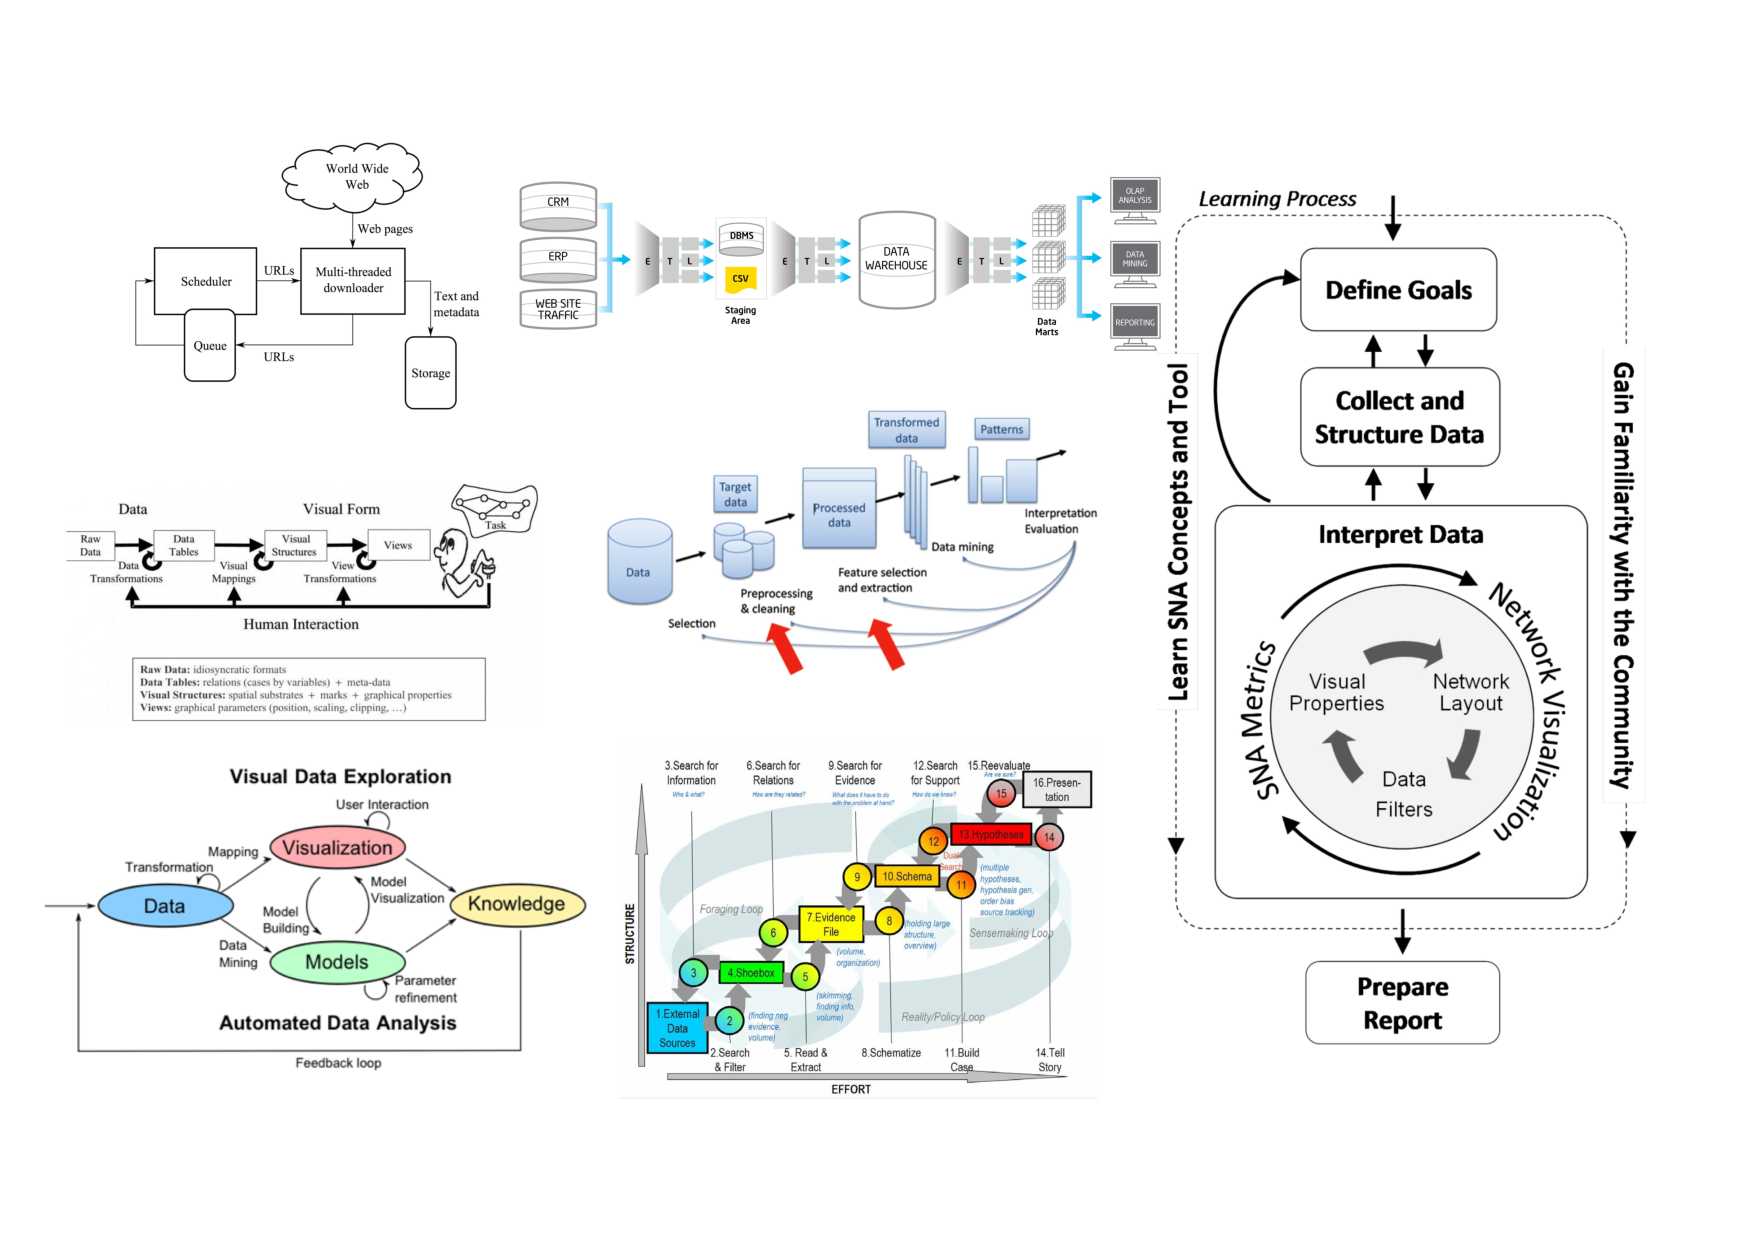
\includegraphics[width=14cm]{figure/Process-models-collage.pdf}
\caption{Process models related to data-driven visual network analytics. The six small diagrams, from top-left: 
web crawling \citep{Wikipedia.org2015}, 
Extract-Transform-Load \citep{Intel2013}, 
information visualization reference model \citep{Card1999ReadingsThink}, 
knowledge extraction from databases \citep{Indarto2013}, 
visual analytics \citep{Keim2010MasteringAnalytics}, 
sensemaking \citep{Pirolli2005TheAnalysis}. 
On the right: Network Analysis and Visualization (NAV) model \citep{Hansen2012DoData}.}
\label{fig:process-model-collage}
\end{figure}

Component-based data-processing pipelines, a technical application of the information visualization reference model, introduce a viable approach for developing reusable pieces of software to support the automation of processes related to social network analysis across application domains \citep{Nykanen2008,Huhtamaki2010Context-DrivenCo-Creation}. To support investigating the social structure among wiki co-creators, for example, \cite{Huhtamaki2010Context-DrivenCo-Creation} present a set of components and a process model for the orchestrated use of the components. A key benefit of the component-based approach \citep{Nykanen2008} is the possibility to integrate existing software tools implemented in different technologies into the data-processing pipeline, given that they can be operated from the command line. The main restriction of the approach is the need to implement the automation through scripting, i.e. writing program code that describes rules for a particular functionality rather than operating a user interface.

The general sensemaking model \citep{Pirolli2005TheAnalysis} divides the sensemaking process into two loops, the foraging loop and the sensemaking loop. To simplify, data is first collected and refined and then transformed into a selection of visualizations and other representations that support sensemaking. The process is iterated as many times as required. Similarly, the process of visual analytics ``typically progresses in an iterative process of view creation, exploration, and refinement'' \citep{Heer2012InteractiveAnalysis}. 

The sensemaking part of the process can be implemented in different ways from purely manual processes where human investigators interact with various user interfaces to conduct the analysis to automated dashboard-centric information systems in which data are collected and processed in runtime. Sensemaking also includes the process of visual analytics \citep{Wong2004VisualAnalytics,Keim2010MasteringAnalytics} that, by default, relies on the availability of software and tools supporting the users. \cite{Heer2012InteractiveAnalysis} give an insightful overview to the specific functionalities that users should be able to operate: 1) specify data and views, 2) manipulate views, and 3) process and provenance their findings.

\cite{Peng2009} builds his definition of reproducible research on three categories: a piece of research is fully reproducible if both the data and code used to are available and, moreover, if the code is executable by anyone. As \cite{Ghosh2013} shows, reproducibility can be approached at many different levels from research policy to detailed technological solutions. Over the last few years, open research practices has become a priority e.g. in Finnish universities\footnote{Open Science and Research at TUT, \url{http://www.tut.fi/en/library/open-science-and-research-data/open-science-at-tut/index.htm}}.

To conclude the review, we note that many of the existing process models are either very general or focus on particular parts of the process. A data-driven visual network analytics approach insists on drawing from a number of process models. For example the use of parallel data sources is often not considered in the process models. Moreover, network analytics introduces specific requirements to the process, importantly including the possibility to calculate node metrics as additional data quantifying the different structural roles of the nodes.

\section{Requirements from the series of investigations}
\label{sec:processmodelrequirements}

Through the series of investigations included in this dissertation, we have shown that visual network analytics is a value-adding approach in exploring and investigating innovation ecosystems and in sharing the findings to others. According to our experience, many of the process-related requirements stemming from the individual investigations are similar. At the same time, many of the investigation-specific analysis processes have insisted us to tailor the process as we have iterated toward the final analysis.

With the data-driven approach, the investigators of innovation ecosystems are able to move fast in the beginning of the process. As the ways of visualizing and investigating a particular phenomenon matures, the investigators may wish continue to follow the phenomena with the support of close to real-time dashboards adding transparency and supporting e.g. longitudinal investigations. The option for automating the process also supports developing these investigative tools toward end-user products for avid innovation ecosystem actors, orchestrators, investigators and policy makers.

The requirements that emerge through the investigations allow us to make way to the third and most important part of results of this dissertation, namely the process model for data-driven visual network analytics. This will answer \ref{objective:processmodel}. This section provides a synthesis of the requirements stemming from the investigations presented in Chapter~\ref{ch:experiments}.

Developed through several rounds of iterations following the Building-Intervention-Evalution cycle \citep{Sein2011ActionResearch}, the core guidelines and requirements for the data-driven visual network analytics process model include the following: enabling manual steps; exploration; transparency; low entry barrier; interoperability; loose coupling; reproducibility; automation;   and continuous data collection. In this dissertation, the requirements presented in this chapter and originally in \ref{pub:ostinato} serve as a design rationale to support the definition of the process model for data-driven visual network analytics, the Ostinato Model. Chapter~\ref{ch:ostinato} describes the model in detail. The next sections introduces each requirement.

% \begingroup
% \captionof{table}{Details on collecting and processing data for the experiments}\label{tab:processreqs}
% \begin{tabular}{p{3cm} p{1cm} p{3cm} p{2cm} p{2cm}}
% \toprule
% Requirement	& Order & Description & Experiment & Origin \\
% \midrule

% Enabling manual steps&1 & & & \\			
% Exploration&2& & & \\
% Transparency&3& & & \\		
% Low entry barrier&4& & & \\		
% Interoperability&5& & & \\	
% Loose coupling&6& & & \\
% Reproducibility&7& & & \\	
% Automation&8& & & \\
% Continuous data collection&9& & & \\

% \bottomrule
% \end{tabular}
% \endgroup

% Table \ref{tab:processreqs} %\href{https://docs.google.com/spreadsheets/d/1o8bqFOYRtAzwMaFiPXr7IrWCoCs77nl7P921AsV3iE8/edit?usp=sharing}{Process model requirements} 
% gives an overview of process model requirements and specifies the experiment in which it was first identified.

\subsection{Enabling manual steps}

While reproducibility is an important long-term objective, at the same time it is key to realize that automating some of the steps may not be feasible when an analysis is conducted the first time or requires intensive tailoring. Therefore, the process should support implementing any of the individual process steps manually. The use of file-based intermediary results is a practical solution in enabling manual analysis steps \citep[cf.][]{Huhtamaki2017ProcessingExperiences}.

\subsection{Exploration}

Visual analytics \citep{Heer2012InteractiveAnalysis} approach is key in enabling users with varied technical skills to collaboratively explore and make sense of a phenomenon. Being able to follow the visual analytics approach, however, requires flexibility from the investigative tools and processes. That is, all the stakeholders of the analysis process should be able to conduct any of the individual steps by themselves even though development of the overall process requires technical development skills.

In the investigations included in this dissertation, we have relied extensively on using Gephi for exploring the networks. At best, however, the whole data processing pipeline from collection to refinement and transformation to visual representation would allow interaction also for non-technical investigators.

\subsection{Transparency}

Developers with extensive technical skills may select to manage the network analysis data throughout the analysis process with a database. Graph databases in particular are appealing for conducting network investigations. To accomplish transparency and flexibility in the process, however, other members of the investigative team will benefit from the option to access the data as files. The use of intermediary results is key in facilitating the transparency and flexibility of the process. Intermediary results refer to data in between the individual steps of the analysis. These data should be available as files in widely used formats, such as CSV and GEXF. In addition to the enhanced transparency, these intermediary results allow for speeding up the analysis process by using cached versions of source data and intermediary results when they have not changed.

\subsection{Low entry barrier}

Analysis of innovation ecosystems and other network-based investigations of complex phenomena require extensive domain knowledge, and hence insist on active participation from domain experts (often without extensive technical expertise) throughout the analysis process. This requirement further underlines the need for transparency of the individual steps of the analysis process.

\subsection{Interoperability} 

Despite the clear benefits of an integrated all-in-one tool for data-driven visual network analytics \citep[cf.][]{Freeman2000VisualizingNetworks}, there will always exist individual tools that offer features not included in the all-in-one tool. Therefore, the investigative team should be able to use a number of existing analytics tools with high usability and rich interactivity including Gephi, NodeXL, KNIME and Tableau for conducting the individual parts of the analysis. Moreover, provisioning the visualized networks and other outputs of the analysis should be possible through dashboard built with Web technologies such as D3.js, DC.js, GEXF.js and the likes. 

\subsection{Loose coupling} 

At best, data-processing pipelines can be built with a range of tools and components implemented in different technologies. Loose coupling is key in enabling this kind of flexibility that allows the introduction and use of new expressive tools from individual software components to full-featured applications as they become available to the investigative team. Many of the tools introduce new opportunities for advancing the analysis process but generally it is not possible to integrate these tools to a data-processing framework in program code, i.e. in native application programming interface level.

Data collection and pre-processing routines in the investigations described in Chapters~\ref{ch:experiments} and \ref{ch:ecosystemnetworks} are implemented in Python using a collection of software modules for additional expressiveness. In addition, we use OpenRefine for cleaning data and Gephi for laying out the networks and calculating some of the network metrics. In addition, we use NetworkX to calculate network metrics in Python for automation. For larger networks, we point to Snap.py\footnote{Snap.py - SNAP for Python, \url{http://snap.stanford.edu/snappy/}}. Being able to use third-party routines for calculating different state-of-the-art network metrics presents an example of extendability that an investigative team will benefit. Tableau allows for visual analytics with a user interface and therefore serves as an example of a tool that many of the investigative teams will use due to loose coupling. 

\subsection{Reproducibility}

In the data-driven visual network analytics approach, reproducibility is first and foremost a technical quality of the process: the investigative team should be able to repeat an investigation or one or more parts of the analysis process and reproduce the results. Reasons for the need to rerun the process include, among others, updates on the source data, development steps of the analysis process, and the introduction of completely new processing steps as well as new tools that insist on the use of a particular data format or extending the existing data. Moreover, dynamic sensemaking for complex phenomena mandates being able to refresh the data and derive new results with updated data. Reproducibility at this technical level also allows the investigative team to release the process, data and results to other researchers interested in the phenomena under investigation.

\subsection{Automation}

Being able to develop automatically updating dashboards as needed gives the investigative team the opportunity to continue observing a particular phenomena of interest over time. It is expected that production-ready analysis processes for dashboards will operate without supervision; however, in the context of exploratory research, some requirements may be relaxed. 

Automation is a key requirement should one decide to implement a dashboard for an up-to-date view into the structure of Demola, EIT Digital, Tekes Young Innovative Companies program or the Finnish innovation ecosystem.

\subsection{Continuous data collection}

Persistent processes for collecting data are often needed, particularly when the investigators wish to tap into social media to capture both the structure and structural dynamics of a phenomenon. Twitter, for example, currently provides only limited access to its historical data, and even then data on followers and friend connections between users do not include timestamps. At times, collecting the data takes days or weeks or ``forever'' to complete, due to throttling or other technical limitation or the sheer size or the dynamic nature of source data.

While the collection process of the Innovation Ecosystems Network Dataset \citep{Rubens2010LeveragingMoves} falls outside of the scope of this dissertation, we want to point that out as an example of a data-collection process that has to run continuously in order to keep the views into innovation ecosystems up to date. 
